% === T19 - Administración de Memoria ===
% David Alejandro Gonzalez Marquez
% fokerman@gmail.com
% https://github.com/fokerman/computingSystemsCourse

\documentclass[aspectratio=169]{beamer}
\usepackage{../packages}

\usepackage{keystroke}
\usepackage{menukeys} 

\title{\Huge Administración de Memoria}
\author{David Alejandro González Márquez}
\institute{}

\date{}

\begin{document}

\begin{frame}[plain]
    \titlepage
    \begin{textblock}{100}(30,80)
    \begin{tcolorbox}[size=small,width=\textwidth,colback={gray!30},title={}]
    \begin{center}
     \scriptsize Clase disponible en: \url{https://github.com/fokerman/computingSystemsCourse}
    \end{center}
    \end{tcolorbox}
    \end{textblock}
%     \begin{textblock}{140}(10,70)
%     \textcolor{rojo}{
%     \textbf{Atención}: La clase será grabada por el anfitrión para su posterior y eventual uso académico dentro de nuestra institución. Su participación en la clase implica brindar su consentimiento para participar en la grabación, aunque pueden mantener su video apagado.}
%     \end{textblock}
\end{frame}

\begin{frame}[t]{Administración de Memoria}
    Los primeros sistemas eran \textbf{monotarea} y la administración de la memoria era muy simple.
    \begin{itemize}
    \item[] Un rango de memoria correspondía al \textcolor{naranjauca}{\textbf{sistema operativo}}
    \item[] y otro rango se asignaba al \textcolor{naranjauca}{\textbf{proceso en ejecución}}.
    \end{itemize}
    \begin{textblock}{100}(20,31) \only<2->{\includegraphics[scale=0.6]{img/monoprograma-layer3.pdf}} \end{textblock}
    \begin{textblock}{100}(50,31) \only<3->{\includegraphics[scale=0.6]{img/monoprograma-layer2.pdf}} \end{textblock}
    \begin{textblock}{100}(80,31) \only<4->{\includegraphics[scale=0.6]{img/monoprograma-layer1.pdf}} \end{textblock}
    \begin{textblock}{37}(110,35)
    \uncover<4->{
    \begin{tcolorbox}[size=small,width=\textwidth,colback={gray!30},title={}]
    \scriptsize Es posible ubicar al Sistema Operativo en la memoria alta como en la memoria baja.\\
    Incluso, podemos tener parte del sistema en ROM mapeado a memoria.
    \end{tcolorbox}
    }
    \end{textblock}
    \begin{textblock}{140}(10,72)
    \only<5->{ 
    \begin{center}
    \textcolor{verdeuca}{Para soportar múltiples tareas tenemos que contar con mecanismos para que\\
    el sistema operativo \textbf{administre la memoria} de cada tarea individualmente.}
    \end{center}
    }
    \end{textblock}
\end{frame}

\begin{frame}[t]{Soporte en hardware}
    \begin{textblock}{110}(42,12)
    \small
    Hasta el momento las direcciones de memoria a las que accede el CPU son las mismas que llegan a la memoria física.\\
    Con este limitado soporte, el sistema operativo solo puede \textbf{asignar áreas de memoria} a los distintos procesos.\\
    \medskip
    \uncover<2->{
    \footnotesize
    Problema de \textcolor{naranjauca}{\textbf{reubicación}}:\\
    \textcolor{verdeuca}{No conocemos donde vamos a cargar el programa en tiempo de generación de código.}\\
    Problema de \textcolor{naranjauca}{\textbf{protección}}:\\
    \textcolor{verdeuca}{No podemos impedir que un proceso escriba la memoria de otro proceso.}\\
    }
    \small
    \medskip
    \uncover<3->{
    \textcolor{verdeuca}{\textbf{Este tipo de soporte se limita a sistemas embebidos.}}\\
    }
    \medskip
    \uncover<4->{
    Los procesadores avanzados cuentan con Unidad de Gestión de Memoria (\texttt{MMU}).\\
    Esta se encarga de \textbf{traducir} las direcciones.\\
    \footnotesize
    Las direcciones que ve el proceso se denominan \textcolor{naranjauca}{\textbf{lógicas}}.\\
    Las direcciones que recibe la memoria se denominan \textcolor{naranjauca}{\textbf{físicas}}.\\
    }
    \small
    \medskip
    \uncover<5->{
    Vamos a ver dos mecanismos de hardware:\\
    \hspace*{1cm}\textcolor{naranjauca}{Segmentación o \emph{relocation register}} y\\
    \hspace*{1cm}\textcolor{naranjauca}{Paginación}
    }
    \end{textblock}
    \begin{textblock}{140}(5,13)
    \includegraphics[scale=0.6]{img/MMU-layer1.pdf}
    \end{textblock}
    \begin{textblock}{140}(5,52)
    \uncover<4->{\includegraphics[scale=0.6]{img/MMU-layer2.pdf}}
    \end{textblock}
\end{frame}

\begin{frame}[t]{Gestión de memoria por Segmentos (\emph{relocation register})}
    \begin{textblock}{120}(45,12)
    El procesador provee un mecanismo que consta de dos registros.\\
    \medskip
    {\hspace*{1cm}}\textcolor{naranjauca}{\textbf{base}}: Indica donde comienza la memoria del proceso.\\
    {\hspace*{1cm}}\textcolor{naranjauca}{\textbf{límite}}: Indica el tamaño de la memoria de proceso.
    \end{textblock}
    \begin{textblock}{100}(10,10)
    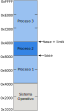
\includegraphics[scale=0.7]{img/proceso_base_limite.pdf}
    \end{textblock}
    \begin{textblock}{85}(60,32)
    \uncover<2->{
    \begin{tcolorbox}[size=small,width=\textwidth,colback={gray!30},title={}]
    \small En el ejemplo el registro base vale \texttt{0x8000} y límite \texttt{0x2000}.\\
    Las direcciones lógicas del Proceso 2\\ comienzan en \texttt{0x0000} y terminan en \texttt{0x1FFF}.\\
    Estas se \textbf{mapean} a la memoria física entre \texttt{0x8000} y \texttt{0xBFFF}.
    \end{tcolorbox}
    }
    \end{textblock}
    \begin{textblock}{120}(45,55)
    \uncover<3->{
    Con este mecanismo podemos asignar cualquier rango de memoria\\ física a cualquier proceso.\\
    \medskip
    Las direcciones lógicas siempre comenzarán en cero y se extenderán\\ hasta el tamaño de la memoria del proceso.\\
    \medskip
    \textcolor{verdeuca}{Los rangos de memoria asignados deben ser contiguos en memoria.}
    }
    \end{textblock}
\end{frame}

\begin{frame}[t]{Gestión de memoria por Segmentación (\emph{relocation register})}
    El funcionamiento consiste en verificar que la dirección lógica que \textbf{no exceda el límite}.\\
    \medskip
    Para luego \textbf{suma el registro de desplazamiento} a la dirección lógica,\\
    \medskip
    obteniendo así la \textbf{dirección física}.\\
    \begin{textblock}{100}(30,30)
    \includegraphics[scale=0.9]{img/logica_a_fisica-layer2.pdf}
    \end{textblock}
    \begin{textblock}{120}(10,74)
    Si la dirección lógica es mayor que el límite,\\ entonces se genera un error de protección.
    \end{textblock}
\end{frame}

\begin{frame}[t]{Gestión de memoria por Segmentación}
    \begin{textblock}{50}(8,12)
    Para implementar múltiples procesos con este mecanismo, se tiene una tabla de segmentos o de registros de desplazamiento y registros de límite.\\
    \medskip
    \textcolor{verdeuca}{Esta tabla es administrada por el sistema operativo y carga los registros cada vez que una tarea distinta es ejecutada.}\\
    \medskip
    \uncover<4->{
    \textcolor{naranjauca}{\textbf{¿Qué sucede si un proceso necesita más memoria?\\ \medskip ¿Cómo se utiliza la memoria libre entre procesos?}}
    }
    \end{textblock}
    \begin{textblock}{100}(48,15) \only<1->{\includegraphics[scale=0.7]{img/paginacion_vs_segmentacion-layer1.pdf}} \end{textblock} % segmentacion
    \begin{textblock}{100}(48,15) \only<2->{\includegraphics[scale=0.7]{img/paginacion_vs_segmentacion-layer2.pdf}} \end{textblock} % P1
    \begin{textblock}{100}(48,15) \only<3->{\includegraphics[scale=0.7]{img/paginacion_vs_segmentacion-layer3.pdf}} \end{textblock} % P2
    \begin{textblock}{100}(48,15) \only<4->{\includegraphics[scale=0.7]{img/paginacion_vs_segmentacion-layer4.pdf}} \end{textblock} % P3
\end{frame}

\begin{frame}[t]{Gestión de memoria por Segmentación}
    \small Con este mecanismo podemos ir asignando rangos de direccionamiento a procesos:
    \begin{textblock}{100}(10,18)  \only<2->{\includegraphics[scale=0.5]{img/fragmentacion-layer2.pdf}} \end{textblock}
    \begin{textblock}{100}(47,18)  \only<3->{\includegraphics[scale=0.5]{img/fragmentacion-layer3.pdf}} \end{textblock}
    \begin{textblock}{100}(84,18)  \only<4->{\includegraphics[scale=0.5]{img/fragmentacion-layer4.pdf}} \end{textblock}
    \begin{textblock}{100}(121,18) \only<5->{\includegraphics[scale=0.5]{img/fragmentacion-layer5.pdf}} \end{textblock}
    \begin{textblock}{100}(10,53)  \only<6->{\includegraphics[scale=0.5]{img/fragmentacion-layer6.pdf}} \end{textblock}
    \begin{textblock}{120}(45,53)  
    \uncover<6->{
    \footnotesize
    \textcolor{verdeuca}{A pesar de tener espacio suficiente, no podemos cargar el nuevo proceso.}\\
    Decimos entonces que nuestra memoria está \textcolor{naranjauca}{\textbf{fragmentada}}.\\
    Se puede dar:\\
    \scriptsize
    \hspace*{0.5cm}\textcolor{naranjauca}{\textbf{fragmentación externa}}: Cuando se da entre memoria de distintos procesos.\\
    \hspace*{0.5cm}\textcolor{naranjauca}{\textbf{fragmentación interna}}: Cuando se da dentro de un proceso.\\
    \medskip
    \footnotesize
    Podemos solucionar este problema \textcolor{naranjauca}{\textbf{compactando la memoria}}.\\
    Pero no resulta una solución practica por su \textbf{gran costo temporal}.
    }
    \end{textblock}
\end{frame}

\begin{frame}[t]{Gestión de memoria por Paginación}
    \uncover<1->{El espacio de direccionamiento lógico se divide en \textcolor{naranjauca}{\textbf{paginas}} de tamaño fijo.\\}
    \uncover<2->{El espacio de direccionamiento físico se divide en \textcolor{naranjauca}{\textbf{marcos}} o \textcolor{naranjauca}{\textbf{frames}} del tamaño de las paginas.\\}
    \begin{textblock}{100}(15,25) \only<1->{\includegraphics[scale=0.7]{img/ejemplo_paginacion-layer1.pdf}} \end{textblock} % logico
    \begin{textblock}{100}(15,25) \only<2->{\includegraphics[scale=0.7]{img/ejemplo_paginacion-layer2.pdf}} \end{textblock} % fisico
    \begin{textblock}{100}(15,25) \only<3->{\includegraphics[scale=0.7]{img/ejemplo_paginacion-layer3.pdf}} \end{textblock} % mmu
    \begin{textblock}{100}(15,25) \only<4->{\includegraphics[scale=0.7]{img/ejemplo_paginacion-layer4.pdf}} \end{textblock} % tabla
    \begin{textblock}{100}(15,25) \only<5->{\includegraphics[scale=0.7]{img/ejemplo_paginacion-layer5.pdf}} \end{textblock} % tabla flechas
    \begin{textblock}{100}(15,25) \only<6->{\includegraphics[scale=0.7]{img/ejemplo_paginacion-layer6.pdf}} \end{textblock} % tabla entradas
    \begin{textblock}{100}(15,25) \only<7->{\includegraphics[scale=0.7]{img/ejemplo_paginacion-layer7.pdf}} \end{textblock} % page 2
    \begin{textblock}{100}(15,25) \only<8->{\includegraphics[scale=0.7]{img/ejemplo_paginacion-layer8.pdf}} \end{textblock} % page 3
    \begin{textblock}{100}(15,25) \only<9->{\includegraphics[scale=0.7]{img/ejemplo_paginacion-layer9.pdf}} \end{textblock} % page 4
    \begin{textblock}{100}(15,25) \only<10->{\includegraphics[scale=0.7]{img/ejemplo_paginacion-layer10.pdf}} \end{textblock} % page 7
    \begin{textblock}{100}(15,25) \only<11->{\includegraphics[scale=0.7]{img/ejemplo_paginacion-layer11.pdf}} \end{textblock} % page 11
    \begin{textblock}{100}(15,25) \only<12->{\includegraphics[scale=0.7]{img/ejemplo_paginacion-layer12.pdf}} \end{textblock} % page 12
    \begin{textblock}{100}(15,25) \only<13->{\includegraphics[scale=0.7]{img/ejemplo_paginacion-layer13.pdf}} \end{textblock} % page 14
    \begin{textblock}{100}(15,25) \only<2->{\includegraphics[scale=0.7]{img/ejemplo_paginacion-layer14.pdf}} \end{textblock} % tamaño
    \begin{textblock}{40}(115,35)
    \uncover<2->{
    \begin{tcolorbox}[size=small,width=\textwidth,colback={gray!30},title={}]
    \small El tamaño de una página suele ser de 4 KB, es decir 4096 Bytes.
    \end{tcolorbox}
    }
    \end{textblock}
    \begin{textblock}{60}(95,65)
    \uncover<13->{La \texttt{MMU} utiliza una tabla que contiene las traducciones para llegar de una página, al marco de página correspondiente
    (\textcolor{naranjauca}{\textbf{tabla de páginas}}).}
    \end{textblock}
\end{frame}

\begin{frame}[t]{Gestión de memoria por Paginación}
    \begin{textblock}{140}(10,12)
    En paginación, las direcciones lógicas se dividen en dos partes,
    el \textcolor{naranjauca}{\textbf{índice de la página}} (\emph{page})\\
    y el \textcolor{naranjauca}{\textbf{desplazamiento}} (\emph{offset}).
    \end{textblock}
    \begin{textblock}{100}(15,10)
    \includegraphics[scale=0.9]{img/logica_a_fisica-layer5.pdf}
    \end{textblock}
    \begin{textblock}{140}(10,50) 
    La traducción de \textbf{page} a \textbf{frame} se realiza por medio de la tabla de páginas,
    la cual se encuentra \textbf{ubicada en memoria}, y es accedida por el procesador para todos los accesos a memoria.\\
    \medskip
    \textcolor{verdeuca}{Es decir, por cada dirección de memoria que el proceso quiera leer o escribir, se debe utilizar la máquinaria de la \texttt{MMU} 
    para traduccir la dirección lógica que ve el proceso a la dirección física que requiere el sistema.}
    \end{textblock}
\end{frame}

\begin{frame}[t]{Gestión de memoria por Paginación}
    Se utiliza como \textcolor{verdeuca}{\textbf{desplazamiento}} dentro de la tabla de páginas el valor de \texttt{P} (\emph{page}).\\
    \medskip
    Dentro de la tabla se toma el valor \texttt{F} (\emph{frame}) y se construye la \textcolor{verdeuca}{\textbf{dirección física}}.\\
    \medskip
    El tamaño de \texttt{P} y \texttt{F} no es necesariamente del mismo.\\
    \begin{textblock}{100}(15,25)
    \includegraphics[scale=0.9]{img/logica_a_fisica-layer3.pdf}
    \end{textblock}
    \begin{textblock}{140}(10,75)
    Si dentro de la tabla, no se encuentra un valor valido, se genera un error de protección.\\
    Este error se conoce como \textcolor{naranjauca}{\textbf{page-fault}}.
    \end{textblock}
\end{frame}

\begin{frame}[t]{Gestión de memoria por Paginación}
    \begin{textblock}{60}(8,15)
    \small
    Cada proceso tendrá su propia tabla de páginas en memoria.\\
    \medskip
    Asignando así páginas lógicas a marcos de página físicos según requiera cada proceso.\\
    \medskip
    \uncover<5->{\textcolor{verdeuca}{El Sistema Operativo utilizará información adicional para
    mantener registro de que páginas de memoria están asignadas
    realmente y cuales están solicitadas pero aun no asignadas.\\}}
    \bigskip
    \uncover<6->{Si bien este mecanismo es \textcolor{naranjauca}{más complejo a nivel de hardware}, resulta más flexible y simple de implementar a nivel de software.\\}
    \medskip
    \uncover<6->{\textcolor{naranjauca}{Evitando además la fragmentación externa.}}
    \end{textblock}    
    \begin{textblock}{100}(60,2) \only<1->{\includegraphics[scale=0.7]{img/paginacion_vs_segmentacion-layer5.pdf}} \end{textblock} % paginacion
    \begin{textblock}{100}(60,2) \only<2->{\includegraphics[scale=0.7]{img/paginacion_vs_segmentacion-layer6.pdf}} \end{textblock} % P1
    \begin{textblock}{100}(60,2) \only<3->{\includegraphics[scale=0.7]{img/paginacion_vs_segmentacion-layer7.pdf}} \end{textblock} % P2
    \begin{textblock}{100}(60,2) \only<4->{\includegraphics[scale=0.7]{img/paginacion_vs_segmentacion-layer8.pdf}} \end{textblock} % P3
\end{frame}

\begin{frame}[t]{Gestión de memoria por Paginación}
    \begin{textblock}{68}(8,12)
    \small
    Cada entrada de una tabla de paginación consiste en un campo \textbf{\emph{frame}} y bits de \textbf{atributos}.\\
    \medskip
    Los bits de atributos pueden ser de \textbf{protección},\\ de \textbf{permisos}, de \textbf{estado} y de \textbf{validez}.\\
    \bigskip
    En el ejemplo, la tabla tiene 3 bits de \emph{frame} y 1 bit de validez.
    \textcolor{verdeuca}{Si indica 1, el campo \emph{frame} es válido.\\}
    \medskip
    \uncover<7->{
    \textcolor{gray}{La dirección lógica tiene 9 bits, de los cuales 5 corresponden al offset, dando un tamaño de página de 32 bytes.}\\
    \medskip
    \textcolor{gray}{Cada entrada de la tabla mínimamente ocupa un byte, por lo tanto nuestra tabla ocupa 16 bytes.}\\
    \medskip
    \textcolor{gray}{El espacio direccionable lógico es de 512 bytes, mientras que físicamente se cuenta con 256 bytes de memoria.}
    }
    \end{textblock}
    \begin{textblock}{100}(80,12) \only<1->{\includegraphics[scale=0.7]{img/paginacion_ejemplo-layer1.pdf}} \end{textblock}
    \begin{textblock}{100}(80,12) \only<2->{\includegraphics[scale=0.7]{img/paginacion_ejemplo-layer2.pdf}} \end{textblock}
    \begin{textblock}{100}(80,12) \only<3->{\includegraphics[scale=0.7]{img/paginacion_ejemplo-layer3.pdf}} \end{textblock}
    \begin{textblock}{100}(80,12) \only<4->{\includegraphics[scale=0.7]{img/paginacion_ejemplo-layer4.pdf}} \end{textblock}
    \begin{textblock}{100}(80,12) \only<5->{\includegraphics[scale=0.7]{img/paginacion_ejemplo-layer5.pdf}} \end{textblock}
    \begin{textblock}{100}(80,12) \only<6->{\includegraphics[scale=0.7]{img/paginacion_ejemplo-layer6.pdf}} \end{textblock}
    \begin{textblock}{100}(80,12) \only<7->{\includegraphics[scale=0.7]{img/paginacion_ejemplo-layer7.pdf}} \end{textblock}
\end{frame}

\begin{frame}[t]{Gestión de memoria por Paginación}
    \begin{textblock}{68}(8,12)
    Si tenemos una memoria muy grande,\\ \textbf{la tabla de paginas también será grande}.\\
    \medskip
    \textcolor{gray}{Si tenemos varios procesos con tablas grandes en memoria, estaremos invirtiendo mucho espacio en la administración de la memoria.\\}
    \medskip
    Para enfrentar este problema se construyen las tablas \textcolor{naranjauca}{\textbf{multinivel}}.\\
    \uncover<2->{
    \medskip
    \textcolor{gray}{Estas consisten en varios niveles escalonados de tablas, para las cuales solo existirán punteros validos a las siguientes tablas si estas son necesarias.\\}
    \medskip
    Permitiendo así ahorrar espacio y tener en memoria solamente la información útil.
    }
    \end{textblock}
    \begin{textblock}{100}(80,3) \only<2->{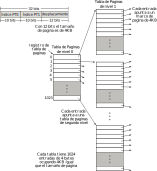
\includegraphics[scale=0.49]{img/paginacion_dos_niveles.pdf}} \end{textblock}
\end{frame}

\begin{frame}[t]{Gestión de memoria por Paginación: Ejemplo de tabla de dos niveles}
    \begin{textblock}{100}(20,10) \only<1->{\includegraphics[scale=0.7]{img/paginacion_ejemplo_nivel_2-layer1.pdf}} \end{textblock}
    \begin{textblock}{100}(20,10) \only<2->{\includegraphics[scale=0.7]{img/paginacion_ejemplo_nivel_2-layer2.pdf}} \end{textblock}
    \begin{textblock}{100}(20,10) \only<3->{\includegraphics[scale=0.7]{img/paginacion_ejemplo_nivel_2-layer3.pdf}} \end{textblock}
    \begin{textblock}{100}(20,10) \only<4->{\includegraphics[scale=0.7]{img/paginacion_ejemplo_nivel_2-layer4.pdf}} \end{textblock}
    \begin{textblock}{100}(20,10) \only<5->{\includegraphics[scale=0.7]{img/paginacion_ejemplo_nivel_2-layer5.pdf}} \end{textblock}
    \begin{textblock}{100}(20,10) \only<6->{\includegraphics[scale=0.7]{img/paginacion_ejemplo_nivel_2-layer6.pdf}} \end{textblock}
    \begin{textblock}{100}(20,10) \only<7->{\includegraphics[scale=0.7]{img/paginacion_ejemplo_nivel_2-layer7.pdf}} \end{textblock}
    \begin{textblock}{100}(20,10) \only<8->{\includegraphics[scale=0.7]{img/paginacion_ejemplo_nivel_2-layer8.pdf}} \end{textblock}
    \begin{textblock}{100}(20,10) \only<9->{\includegraphics[scale=0.7]{img/paginacion_ejemplo_nivel_2-layer9.pdf}} \end{textblock}
\end{frame}

\begin{frame}[t]{Gestión de memoria por Paginación: Ejemplo de tabla de tres niveles}
    \begin{textblock}{100}(18,15) \only<1->{\includegraphics[scale=0.7]{img/paginacion_ejemplo_nivel_3-layer1.pdf}} \end{textblock}
    \begin{textblock}{100}(18,15) \only<2->{\includegraphics[scale=0.7]{img/paginacion_ejemplo_nivel_3-layer2.pdf}} \end{textblock}
    \begin{textblock}{100}(18,15) \only<3->{\includegraphics[scale=0.7]{img/paginacion_ejemplo_nivel_3-layer3.pdf}} \end{textblock}
    \begin{textblock}{100}(18,15) \only<4->{\includegraphics[scale=0.7]{img/paginacion_ejemplo_nivel_3-layer4.pdf}} \end{textblock}
    \begin{textblock}{100}(18,15) \only<5->{\includegraphics[scale=0.7]{img/paginacion_ejemplo_nivel_3-layer5.pdf}} \end{textblock}
    \begin{textblock}{100}(18,15) \only<6->{\includegraphics[scale=0.7]{img/paginacion_ejemplo_nivel_3-layer6.pdf}} \end{textblock}
    \begin{textblock}{100}(18,15) \only<7->{\includegraphics[scale=0.7]{img/paginacion_ejemplo_nivel_3-layer7.pdf}} \end{textblock}
    \begin{textblock}{100}(18,15) \only<8->{\includegraphics[scale=0.7]{img/paginacion_ejemplo_nivel_3-layer8.pdf}} \end{textblock}
    \begin{textblock}{100}(18,15) \only<9->{\includegraphics[scale=0.7]{img/paginacion_ejemplo_nivel_3-layer9.pdf}} \end{textblock}
    \begin{textblock}{100}(18,15) \only<10->{\includegraphics[scale=0.7]{img/paginacion_ejemplo_nivel_3-layer10.pdf}} \end{textblock}
    \begin{textblock}{100}(18,15) \only<11->{\includegraphics[scale=0.7]{img/paginacion_ejemplo_nivel_3-layer11.pdf}} \end{textblock}
\end{frame}

\begin{frame}[t]{Gestión de memoria por Paginación: TLB}
    \small
    La traducción de una dirección de memoria lleva tiempo.\\
    \textcolor{gray}{Se requiere recorrer todo el árbol de paginación hasta llegar al marco de pagina buscado.}\\
    \medskip
    Para solucionar esto implementamos una memoria caché: \textcolor{naranjauca}{\textbf{TLB (\emph{Translation Lookaside Buffers})}}\\
    \begin{textblock}{100}(15,28)
    \includegraphics[scale=0.9]{img/logica_a_fisica-layer4.pdf}
    \end{textblock}
    \begin{textblock}{100}(10,77)
    Su tarea es encontrar el \emph{frame} a partir de la \emph{page}.\\
    Su implementación es una cache completamente asociativa.
    \end{textblock}
\end{frame}

\begin{frame}{Estructuras de datos para la administración de memoria}
    \begin{textblock}{65}(10,15)
    \small
    Para que es sistema operativo lleve registro de que áreas de memoria están en uso y cuales no, se utilizan estructuras de datos particulares.\\
    \vspace{0.7cm}
    \uncover<2->{En un \textbf{mapa de bits}, cada bit indica si un determinado rango de memoria esta en uso o esta libre.\\}
    \bigskip
    \uncover<3->{Una \textbf{lista enlazada}, deja registro en cada nodo, si se trata de un espacio libre o ocupado.\\
    En esta estructura pueden existir nodos contiguos con áreas ocupadas, pero no libres,\\ ya que estos últimos se colapsan en uno solo.}
    \end{textblock}
    \begin{textblock}{100}(80,15)
    \uncover<2->{\small \textcolor{naranjauca}{\textbf{Estructura de Mapa de bits}}\\ \vspace{0.2cm}
    \includegraphics[scale=0.9]{img/bitmap.pdf} }
    \end{textblock}
    \begin{textblock}{100}(80,50)
    \uncover<3->{\small \textcolor{naranjauca}{\textbf{Estructura de Lista enlazada}}\\ \vspace{0.2cm}
    \includegraphics[scale=0.9]{img/linked_list.pdf} }
    \end{textblock}
\end{frame}

% \begin{frame}{Mecanismos para solicitar memoria}
%     \begin{textblock}{65}(10,15)
%     \small
%     xxxx
%     \end{textblock}
%     \begin{textblock}{100}(80,15)
%     \includegraphics[scale=0.3]{img/procesos_en_memoria-layer1}
%     \end{textblock}
%     \begin{textblock}{100}(80,50)
%     \includegraphics[scale=0.3]{img/procesos_en_memoria-layer2.pdf}
%     \end{textblock}
% %     - como agrandamos el espacio de memoria usado por el programa?
% %     - en segmentacion agrandamos el espacio, siempre que tengamos espacio contiguo que podamos agregar, sino tenemos que mover el programa, lo cual es muy costoso!
% %     - en paginacion es mas simple, 
% \end{frame}

\begin{frame}[t]{Memoria Virtual}
    \small
    Utilizando los mecanismos que provee el procesar para administrar memoria,
    podemos asignar un espacio de memoria independiente a cada proceso.
    \textcolor{verdeuca}{Sin embargo, la memoria física es limitada, y no podemos tener todos
    los procesos simultaneamente en memoria.}\\
    \medskip
    \uncover<2->{Para esto existen los \textcolor{naranjauca}{\textbf{mecanismos de swapping}},
    que permiten guardar temporariamente en almacenamiento secundario las paginas poco utilizadas,
    mientras que las paginas de más demandadas están en memoria.}
    \begin{textblock}{100}(12,43)
    \uncover<2->{\includegraphics[scale=0.6]{img/swapping.pdf} }
    \end{textblock}
    \begin{textblock}{85}(63,40)
    \uncover<3->{\small Conceptos clave en memoria virtual:
    \footnotesize
    \begin{itemize}
     \item \textcolor{verdeuca}{Las direcciones lógicas o virtuales son las que ve el proceso en ejecución, y viven solamente dentro del procesador.}
     \item \textcolor{verdeuca}{Las direcciones físicas son las que llegan a la memoria principal.}
     \item \textcolor{verdeuca}{En almacenamiento secundario se guardan paginas de memoria que fueron remplazadas bajo alguna política de remplazos.}
    \end{itemize}
     Si estamos remplazando paginas todo el tiempo, nuestro sistema puede entrar en \emph{crashing}. }
    \end{textblock}
\end{frame}

\begin{frame}[t]{Memoria Virtual: Resumen}
    \begin{textblock}{100}(3,11)
    \includegraphics[scale=0.75]{img/memoria_virtual.pdf}
    \end{textblock}
\end{frame}

\begin{frame}{Interrupción de Page Fault}
    \small
    La interrupción de fallo de página se produce en tres situaciones.
    \begin{itemize}
     \item El \textcolor{verdeuca}{\textbf{nivel de privilegios}} no es suficiente para acceder.
     \item La acción a realizar {\footnotesize(Read, Write, Execute)} no se corresponde con los \textcolor{verdeuca}{\textbf{permisos de la página}}.
     \item La página \textcolor{verdeuca}{\textbf{no está mapeada}}.
    \end{itemize}
    \pause
    \bigskip
    En cualquiera de los casos se pueden dar dos soluciones en la rutina de atención de la interrupción.
    \begin{itemize}
     \item El acceso es \textbf{incorrecto} y por lo tanto se debe matar al proceso en ejecución.
     \item El acceso es \textbf{correcto} y el sistema operativo debe resolver el problema.
    \end{itemize}
    \pause
    \bigskip
    Esta interrupción tiene un caracter especial, ya que funciona como una \textbf{trampa}.\\
    \medskip
    \textcolor{verdeuca}{Cuando se retorna de la rutina, se vuelve a la instrucción que produjo el error para que\\
    \textbf{continue ejecutando desde el mismo lugar}, pero ahora con la memoria correctamente mapeada.}
\end{frame}

\begin{frame}{Política de optimización \texttt{Copy-On-Write}}
    \begin{textblock}{75}(8,12)
    \small
    Cuando se ejecuta un \texttt{fork}, un proceso nuevo es creado.\\
    \medskip
    \textcolor{gray}{El nuevo proceso existirá en un espacio de memoria nuevo, y para esto se deben \textbf{copiar todas las páginas} del proceso padre, duplicando la memoria ocupada.}\\
    \medskip
    \uncover<2->{Para evitar copiar las páginas, estas se mapean como \textbf{solo lectura para ambos procesos}.\\}
    \medskip
    \begin{center}
    \uncover<3->{\textcolor{verdeuca}{\textbf{Cuando cualquiera de los procesos quiera escribir,\\ se generará un fallo de página}}.\\}
    \end{center}
    \medskip
    \uncover<3->{
    La rutina de atención de interrupciones actuará y determinará que se trata de \textbf{páginas físicas compartidas}.
    Duplicando entonces la memoria en dos páginas físicas distintas.\\}
    \begin{center}
    \uncover<3->{\textcolor{naranjauca}{\textbf{Se mapea una copia en ambos procesos.}}\\}
    \end{center}
    \end{textblock}
    \begin{textblock}{100}(90,5) \only<2->{\includegraphics[scale=1]{img/copy-on-wite-layer1.pdf} } \end{textblock}
    \begin{textblock}{100}(90,5) \only<3->{\includegraphics[scale=1]{img/copy-on-wite-layer2.pdf} } \end{textblock}
\end{frame}

\begin{frame}{Remplazo de páginas}
    \begin{textblock}{70}(10,12)
    \small
    Cuando no hay páginas libres en memoria física donde cargar los nuevos marcos de página.\\
    \textcolor{naranjauca}{Se debe seleccionar una página \textbf{víctima}.\\}
    \medskip
    \uncover<2->{\textcolor{verdeuca}{Esta página será desalojada de memoria y almacenada en almacenamiento secundario.\\}}
    \medskip
    \uncover<3->{La nueva página será cargada en su lugar y se mapeará en la tabla de páginas de la tarea.\\}
    \medskip
    \textcolor{gray}{
    \footnotesize
    \uncover<3->{Los algoritmos de elección de páginas víctima pueden ser: First In First Out (FIFO), Least Recently Used (LRU), Least Frequenly Used (LFU), FIFO Second-chance, etc.\\}}
    \medskip
    \uncover<4->{
    \begin{tcolorbox}[size=small,width=\textwidth,colback={gray!30},title={\emph{dirty-bit}}]
    \footnotesize
    La tabla de páginas contiene además un bit que indica si la página fue modificada. Esto permite optimizar el algoritmo de remplazo, copiando a memoria secundaria solo la página que fue modificada.
    \end{tcolorbox}
    }
    \end{textblock}
    \begin{textblock}{100}(90,7)
    \includegraphics[scale=0.7]{img/remplazo_de_paginas.pdf}
    \end{textblock}
\end{frame}

\begin{frame}[fragile]{Bibliografía}
    \begin{itemize}
        \setlength\itemsep{0.5cm}
        \item[-] \small Tanenbaum, ``Modern Operating Systems'', 4th Edition, 2015.\\
        \begin{itemize}
            \item \textbf{Chapter 3 - Memory Management}, páginas 181-208
        \end{itemize}
        \item[-] \small Silberschatz, ``Fundamentos de Sistemas Operativos'', 7ma Edición, 2006.\\
        \begin{itemize}
            \item \textbf{Capítulo 8 - Memoria principal}, páginas 243-267 y 279-288
        \end{itemize}
    \end{itemize}
\end{frame}

\begin{frame}{Ejercicios}
    \vfill
    Con lo visto, ya pueden resolver todos los ejercicios de la Guía de Administración de Memoria.
    \vfill
\end{frame}

\begin{frame}[plain]
    \begin{center}
    \vspace{2cm}
    \huge ¡Gracias!\\
    \vspace{2cm}
    \normalsize Recuerden leer los comentarios adjuntos\\ en cada clase por aclaraciones.
    \end{center}
\end{frame}

\end{document}
